\subsubsection{Modelo Operating System Actuators}

Nuestra abstracción de un sistema \gls{iot} necesita contar con una serie de elementos que habitualmente encontramos proporcionados por los sistemas operativos.

Para ello necesitamos modelar estos elementos que utilizaremos desde nuestro \gls{dsl}.

Este modelo, representado en la figura  \ref{fig:modelo_operatingsystemactuators_classes}, representa las funcionalidades básicas que necesitamos por parte del sistema operativo para el funcionamiento de nuestros dispositivos \gls{iot}. Cuenta con una muestra de las tareas que podría implementar nuestro \gls{dsl}, tareas de alto nivel tales como: descarga de archivos, ejecución de programas del sistema, visualización de imágenes en pantalla y reproducción de archivos de audio o vídeo.

\begin{figure}[htp]
	\centering
    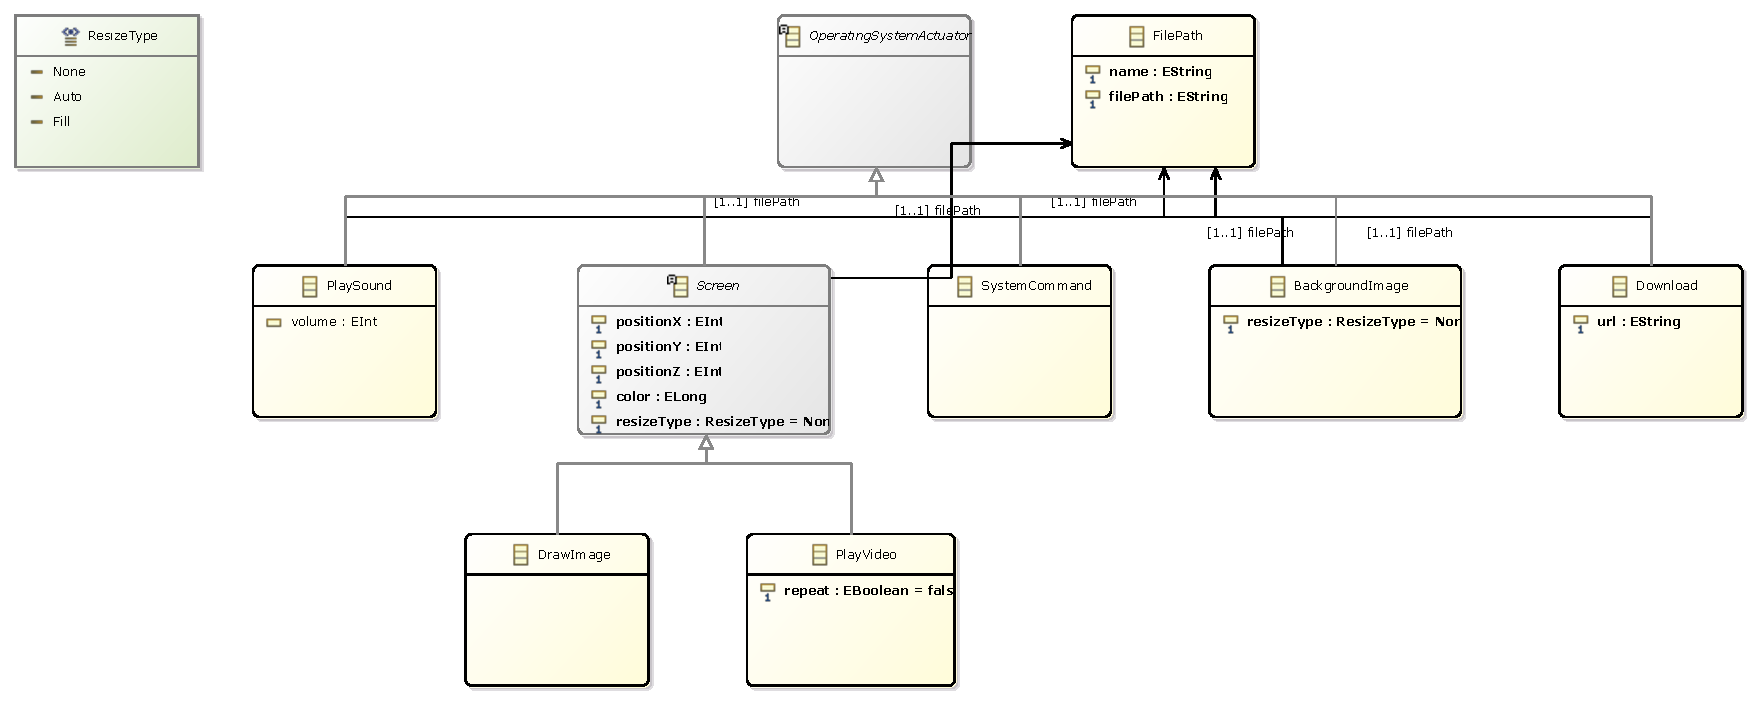
\includegraphics[height=0.3\textheight]{images/models/operatingsystemactuators_class_diagram.pdf}
    \captionmodeloclase{OperatingSystemActuators}
    \label{fig:modelo_operatingsystemactuators_classes}
\end{figure}
